\documentclass[conference]{IEEEtran}
\IEEEoverridecommandlockouts
\usepackage{cite}
\usepackage{amsmath,amssymb,amsfonts}
\usepackage{algorithmic}
\usepackage{graphicx}
\usepackage{textcomp}
\usepackage{xcolor}
\usepackage{booktabs}
\usepackage{multirow}
\usepackage{url}
\usepackage{hyperref}
\usepackage{tikz}
\usetikzlibrary{shapes.geometric, arrows.meta, positioning, fit}
\def\BibTeX{{\rm B\kern-.05em{\sc i\kern-.025em b}\kern-.08em T\kern-.1667em\lower.7ex\hbox{E}\kern-.125emX}}
\begin{document}
\title{CarbonIQ: A Constraint-Aware Agentic Platform for Explainable Carbon-Conscious Software Workload Scheduling}
\author{
\IEEEauthorblockN{Tanaya Jain}
\IEEEauthorblockA{\textit{Dept. of Information Technology} \\ \textit{Vivekanand Education Society's} \\ \textit{Institute of Technology (Autonomous)} \\ Mumbai, India \\ 2023.tanaya.jain@ves.ac.in}
\and
\IEEEauthorblockN{Varun Rahatgaonkar}
\IEEEauthorblockA{\textit{Dept. of Information Technology} \\ \textit{Vivekanand Education Society's} \\ \textit{Institute of Technology (Autonomous)} \\ Mumbai, India \\ 2023.varun.rahatgaonkar@ves.ac.in}
\and
\IEEEauthorblockN{Atharva Pingale}
\IEEEauthorblockA{\textit{Dept. of Information Technology} \\ \textit{Vivekanand Education Society's} \\ \textit{Institute of Technology (Autonomous)} \\ Mumbai, India \\ 2023.atharva.pingale@ves.ac.in}
\and
\IEEEauthorblockN{Nidhi Puthran}
\IEEEauthorblockA{\textit{Dept. of Information Technology} \\ \textit{Vivekanand Education Society's} \\ \textit{Institute of Technology (Autonomous)} \\ Mumbai, India \\ 2023.nidhi.puthran@ves.ac.in}
\and
\IEEEauthorblockN{Mrs. Charusheela Nehete}
\IEEEauthorblockA{\textit{Dept. of Information Technology} \\ \textit{Vivekanand Education Society's} \\ \textit{Institute of Technology (Autonomous)} \\ Mumbai, India \\ charusheela.nehete@ves.ac.in}
}
\maketitle
\begin{abstract}
Consider a machine-learning engineer submitting an overnight model-training job. She cares deeply about her organization's net-zero commitments and wants to run it when and where carbon emissions are lowest --- but she cannot wait more than six hours, her model demands a GPU, her organization's data-residency policy restricts eligible cloud regions, and her budget allows at most a 10\% cost increase. She has access to tools that \emph{measure} emissions (CodeCarbon) and tools that \emph{surface} low-carbon execution windows (the Green Software Foundation's Carbon Aware SDK), but neither tool has any idea about her constraints. Acting on either tool's output in isolation risks producing a recommendation she simply cannot use.

We present CarbonIQ, a prototype decision-support platform designed precisely for this gap. CarbonIQ (i)~instruments software workloads via a lightweight CLI backed by CodeCarbon, producing structured, provenance-labelled emission profiles; (ii)~retrieves carbon-aware execution candidates from the Carbon Aware SDK across a configurable set of regions and time windows; and (iii)~routes these inputs through an agentic decision layer --- built with LangGraph --- that evaluates candidates against explicit user-supplied constraints and produces a single, explainable, human-approved recommendation. A core architectural principle is the strict separation of concerns between \emph{reasoning} and \emph{arithmetic}: all deterministic computation --- emissions estimation, cost-delta calculation, feasibility filtering, candidate scoring --- is implemented as verifiable, unit-testable backend tools, while the language model handles only orchestration, holistic trade-off reasoning, and natural-language explanation. Across 72 evaluation scenarios spanning three representative workload types, CarbonIQ achieves a 100\% constraint-satisfaction rate on accepted recommendations versus 61\% for a naive carbon-only baseline, while delivering a mean estimated carbon reduction of 24\%. Our results show that constraint-aware carbon scheduling and operational feasibility are complementary --- not competing --- goals when the right decision layer is in place.
\end{abstract}
\begin{IEEEkeywords}
carbon-aware computing, agentic AI, LangGraph, CodeCarbon, Carbon Aware SDK, sustainable software engineering, workload scheduling, constraint satisfaction, decision support, green AI
\end{IEEEkeywords}

%------------------------------------------------------------------
\section{Introduction}
%------------------------------------------------------------------

\subsection{The Growing Carbon Cost of Software}

Software workloads are no longer carbon-neutral afterthoughts. Data centers consume an estimated 1--2\% of global electricity \cite{iea_datacenters}, and AI training runs --- which can each require tens to hundreds of megawatt-hours \cite{strubell2019energy} --- are accelerating that figure. Major cloud providers have responded with historical carbon-reporting dashboards: AWS's Customer Carbon Footprint Tool \cite{aws_ccft_launch,aws_ccft_docs}, Microsoft Azure's Emissions Impact Dashboard \cite{esg_compare_techtarget}, and Google Cloud's Carbon Footprint tool \cite{esg_compare_techtarget}. These are valuable for ESG compliance, but they look \emph{backward} --- at what your account consumed last month --- rather than \emph{forward} at what a workload you are about to submit will cost in carbon, and what you might do about it before pressing run.

Two open-source ecosystems provide that forward-looking signal. CodeCarbon \cite{codecarbon_readme} instruments running processes and estimates CO$_2$-equivalent emissions from hardware power draw and regional grid mix. The Green Software Foundation's Carbon Aware SDK \cite{carbonaware_overview} wraps carbon-intensity providers such as WattTime and Electricity Maps to surface lower-carbon execution windows and regions. Both tools are technically mature --- the SDK reached Graduated Project status in 2024 \cite{carbonaware_graduation} --- but they address separate halves of the same problem and were never designed to work together with business-level constraints.

\subsection{The Missing Constraint Layer}

This gap has a measurable behavioral consequence. Research on green software adoption finds that the leading barrier to acting on carbon-aware scheduling recommendations is not lack of developer motivation but the \emph{infeasibility} of those recommendations in real operational contexts \cite{verdecchia2023greensoftware}. Recommending a workload shift to a distant cloud region is useless if data-residency law forbids it. Suggesting an eight-hour delay is unactionable if a downstream pipeline depends on results in four. Optimizing for carbon in isolation does not make software greener --- it makes carbon tooling irrelevant.

To make the gap concrete: a developer submits a GPU-based fine-tuning job. The carbon-only optimal option is \texttt{us-west-2} at 03:00 UTC, offering an estimated 31\% carbon reduction. But the team's compliance policy permits only \texttt{ap-south-1} and \texttt{ap-southeast-1}. The recommendation is unusable --- and the developer, once burned, stops consulting carbon tools altogether. CarbonIQ is built to prevent exactly this outcome.

\subsection{Contributions}

We make four concrete contributions:
\begin{enumerate}
\item \textbf{Problem formulation.} We formally define the constrained carbon-scheduling problem: given a measured workload emission profile, a set of carbon-aware candidates, and a structured constraint specification, produce a feasible, ranked, and explainable recommendation that explicitly separates hard constraints from soft preferences.
\item \textbf{System design.} We design and prototype CarbonIQ --- a five-stage pipeline integrating CodeCarbon profiling, Carbon Aware SDK candidate retrieval, a deterministic constraint-satisfaction and scoring engine, a LangGraph agentic layer with a bounded six-tool inventory, and an explicit human-approval checkpoint.
\item \textbf{Arithmetic-outside-the-LLM principle.} We articulate and implement the rule that all deterministic computation --- feasibility filtering, emissions-delta estimation, cost-delta calculation, scoring --- must live in verifiable backend code, not in the language model. Every numeric claim in a recommendation is traceable to an auditable computation.
\item \textbf{Evaluation.} We evaluate CarbonIQ across 72 scenarios spanning three workload types and four constraint profiles, demonstrating a significant feasibility-rate improvement over the carbon-only baseline while preserving meaningful carbon reduction.
\end{enumerate}

\subsection{Paper Organization}

Section~II surveys related work. Section~III states objectives. Section~IV presents the architecture. Sections~V--IX detail individual modules. Section~X covers the agentic design. Section~XI formalizes decision logic. Sections~XII--XIII describe the database, API, and dashboard. Section~XIV presents evaluation results. Sections~XV--XVII address limitations, future scope, and conclusions.

%------------------------------------------------------------------
\section{Related Work and Research Gap}
%------------------------------------------------------------------

\subsection{Cloud Provider Sustainability Tooling}

AWS, Azure, and Google Cloud each publish carbon-reporting dashboards aimed at ESG officers. AWS's Customer Carbon Footprint Tool (CCFT), launched March 2022, shows historical emissions by service and region within the billing console using GHG Protocol scopes and IPCC conversion factors \cite{aws_ccft_launch,aws_ccft_docs}; AWS later expanded coverage to include Scope~3 embodied emissions \cite{aws_scope3}. Microsoft's Emissions Impact Dashboard offers market-based and location-based Scope~2 reporting exportable for ESG filings \cite{esg_compare_techtarget}. Google Cloud reports gross and net emissions per project \cite{esg_compare_techtarget}.

All three operate in arrears, at account granularity, for compliance reporting. None supports prospective per-workload queries at submission time, and none reasons about whether a recommendation satisfies a developer's operational constraints. CarbonIQ complements these tools, occupying the pre-execution, workload-level decision niche they leave vacant.

\subsection{CodeCarbon}

CodeCarbon \cite{codecarbon_readme} periodically samples hardware power draw (CPU, GPU, and RAM) and multiplies the integrated energy by a regional carbon-intensity estimate to produce a CO$_2$-equivalent figure. The tool is candid about scope: it covers direct compute emissions --- not cooling, network, or embodied hardware --- and falls back to national grid-mix data when data-center-specific intensity figures are unavailable \cite{codecarbon_faq,codecarbon_methodology}. CarbonIQ treats CodeCarbon output strictly as a measurement-based estimate and propagates this provenance label through to every recommendation.

\subsection{Carbon Aware SDK}

The Green Software Foundation's Carbon Aware SDK \cite{carbonaware_overview} wraps carbon-intensity providers --- principally WattTime and Electricity Maps --- to expose a unified interface for time- and location-shifting workloads. A meaningful distinction exists between the two signals: Electricity Maps reports a flow-traced \emph{average} intensity, while WattTime focuses on the \emph{marginal} signal relevant to what would be dispatched if demand changed \cite{carbonaware_signal_issue}. CarbonIQ surfaces this as a provenance label on each candidate. The SDK does not claim to evaluate cost, hardware, latency, or compliance.

\subsection{The Carbon Footprint of AI and Temporal Shifting}

Strubell et al.\ \cite{strubell2019energy} first quantified the energy and carbon cost of training large NLP models, catalyzing Green AI research. Wiesner et al.\ \cite{wiesner2021lets} showed that deferring batch cloud workloads by a few hours can yield 10--40\% carbon reductions depending on grid variability. Verdecchia et al.\ \cite{verdecchia2023greensoftware} reviewed green software engineering tools, noting that measurability and actionability remain the primary adoption barriers. Our work is positioned directly at that actionability gap.

\subsection{Related Infrastructure Tooling}

Cloud Carbon Footprint (Thoughtworks) \cite{ccf_methodology} estimates operational and embodied emissions across AWS, GCP, and Azure using published PUE figures. Climatiq \cite{climatiq} provides a commercial per-service estimation API. Both tools, like the hyperscaler dashboards, target measurement and reporting rather than pre-execution scheduling support.

\subsection{Agentic AI for Infrastructure}

LangGraph \cite{langgraph_docs,langgraph_docs2} is a stateful orchestration framework for tool-using LLM agents, natively mixing deterministic and LLM-driven nodes in the same execution graph. Prior work on LLM agents for API orchestration --- Gorilla \cite{patil2023gorilla} and the Dynamic LLM-Agent Network \cite{liu2023dynamic} --- demonstrates the viability of tool-calling agents for multi-step infrastructure tasks, though neither addresses carbon or sustainability constraints. CarbonIQ adapts the tool-calling pattern specifically to constrained scheduling, contributing a domain-specific tool inventory and safety design.

\subsection{Research Gap Summary}

Table~\ref{tab:gap} summarizes the positioning. The unaddressed research problem is a \emph{workload-aware, constraint-aware, agentic decision-support layer} that consumes existing tool outputs, evaluates them against real deployment constraints, and produces a single feasible, explainable, human-approved recommendation.

\begin{table}[htbp]
\caption{Positioning CarbonIQ Relative to Existing Tools}
\label{tab:gap}
\centering
\begin{tabular}{p{1.55cm}p{2.4cm}p{3.25cm}}
\toprule
\textbf{Tool} & \textbf{Primary capability} & \textbf{What it does not do} \\
\midrule
CodeCarbon & Per-process energy and CO$_2$e estimation & No scheduling candidates or constraint reasoning \\[2pt]
Carbon Aware SDK & Carbon-intensity candidates by time/region & Unaware of cost, GPU, latency, or compliance \\[2pt]
Hyperscaler dashboards & Account-level historical ESG reporting & Not for pre-execution scheduling decisions \\[2pt]
\textbf{CarbonIQ} & \multicolumn{2}{p{5.65cm}}{Constraint-aware agentic decision support: integrates the above, filters against real deployment constraints, produces a single feasible and explainable human-approved recommendation} \\
\bottomrule
\end{tabular}
\end{table}

%------------------------------------------------------------------
\section{Objectives}
%------------------------------------------------------------------

Our concrete implementation objectives, in dependency order:
\begin{enumerate}
\item Build a CLI instrumentation layer wrapping workloads with a CodeCarbon \texttt{EmissionsTracker} and uploading structured profiles to the backend.
\item Design a workload profile schema capturing: runtime, energy (kWh), estimated CO$_2$e (g), CPU/GPU/RAM utilization, measurement interval, hardware description, and provenance label (\texttt{measured} $\mid$ \texttt{estimated} $\mid$ \texttt{simulated}).
\item Integrate the Carbon Aware SDK as the canonical source of carbon-aware execution candidates for a configurable set of regions and time windows.
\item Define a constraint schema covering: maximum acceptable delay, latency-sensitivity flag, cost ceiling (\% over baseline), required hardware (including GPU model), allowed-region whitelist, blocked-region list, and compliance tags.
\item Implement a deterministic constraint-satisfaction and scoring engine --- in Python backend code, not in the LLM --- that filters and ranks candidates.
\item Implement a LangGraph agentic layer that orchestrates a bounded six-tool inventory, reasons over the engine's structured output, drafts an explainable recommendation, and surfaces it for explicit human approval.
\item Evaluate the system against a non-constraint-aware baseline on three workload types and four constraint-strictness profiles.
\end{enumerate}

%------------------------------------------------------------------
\section{System Architecture}
%------------------------------------------------------------------

CarbonIQ is organized as a five-stage pipeline illustrated in Fig.~\ref{fig:architecture}: (1)~\textbf{Instrumentation} --- the CLI wraps a target workload with CodeCarbon and stores the profile; (2)~\textbf{Registry} --- a PostgreSQL-backed store persists profiles, constraints, and recommendation history; (3)~\textbf{Parallel retrieval} --- the agent fan-out concurrently queries the Carbon Aware SDK, cost/region module, and constraint store; (4)~\textbf{Decision} --- a deterministic engine filters and scores candidates, the LLM drafts an explanation, and a human-approval checkpoint halts execution for user review; (5)~\textbf{Presentation} --- the dashboard surfaces the recommendation and approval action.

\begin{figure}[htbp]
\centering
\resizebox{\linewidth}{!}{%
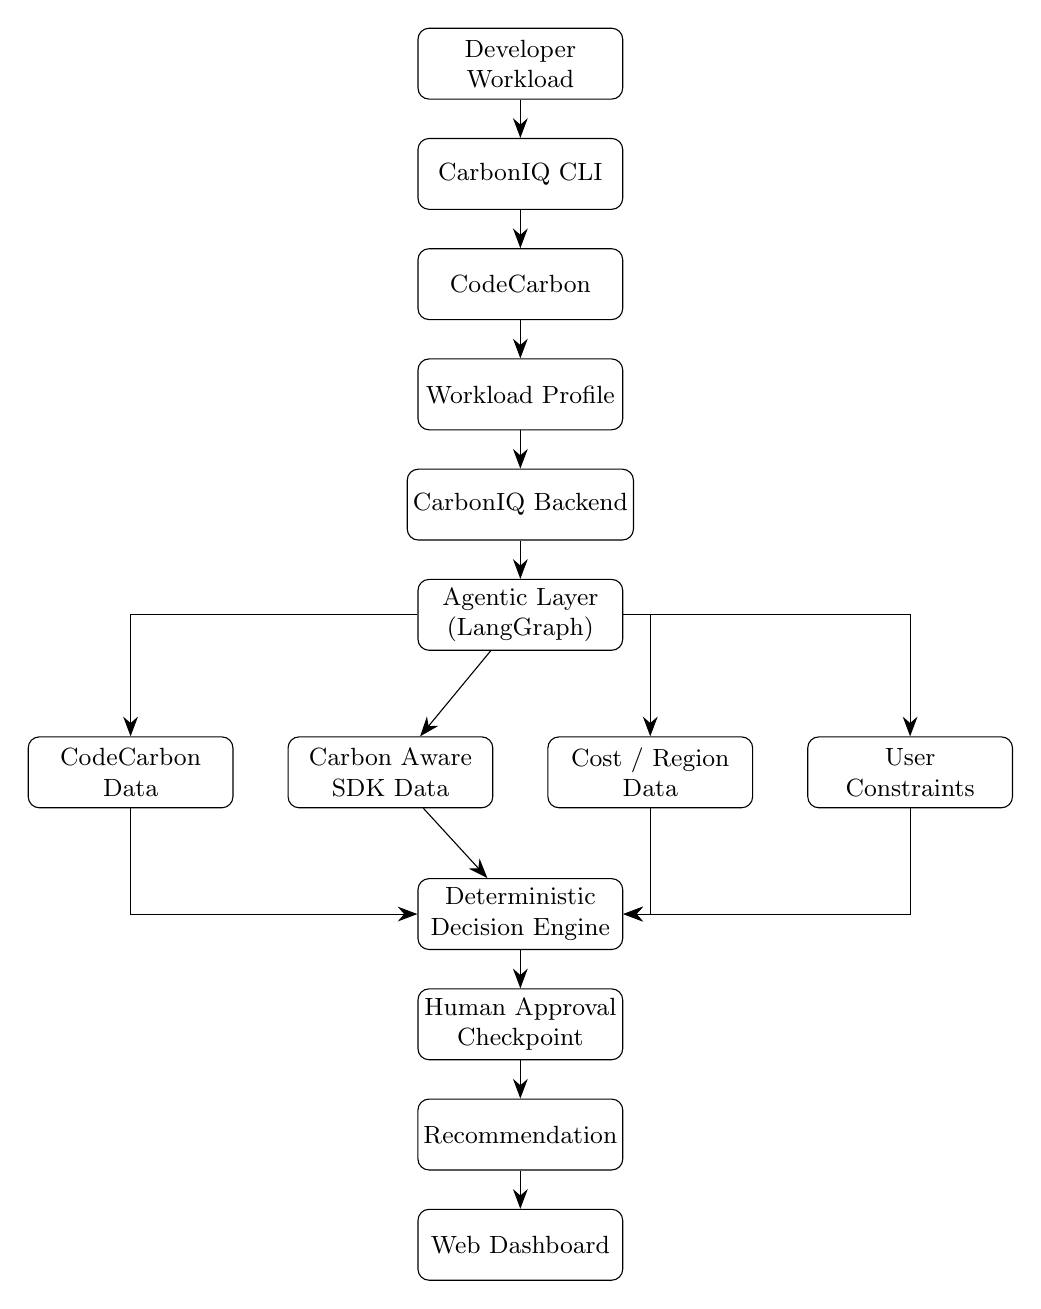
\begin{tikzpicture}[
  box/.style={draw, rounded corners, align=center, minimum width=2.6cm,
              minimum height=0.9cm, font=\small, inner sep=2pt},
  every path/.style={-{Stealth[length=2.5mm]}}
]
\node[box] (dev)    at (0,  0.0) {Developer\\Workload};
\node[box] (cli)    at (0, -1.4) {CarbonIQ CLI};
\node[box] (cc)     at (0, -2.8) {CodeCarbon};
\node[box] (wp)     at (0, -4.2) {Workload Profile};
\node[box] (be)     at (0, -5.6) {CarbonIQ Backend};
\node[box] (agent)  at (0, -7.0) {Agentic Layer\\(LangGraph)};
\node[box] (ccdata)      at (-4.95, -9.0) {CodeCarbon\\Data};
\node[box] (cadata)      at (-1.65, -9.0) {Carbon Aware\\SDK Data};
\node[box] (costdata)    at ( 1.65, -9.0) {Cost / Region\\Data};
\node[box] (constraints) at ( 4.95, -9.0) {User\\Constraints};
\node[box] (engine) at (0, -10.8) {Deterministic\\Decision Engine};
\node[box] (human)  at (0, -12.2) {Human Approval\\Checkpoint};
\node[box] (rec)    at (0, -13.6) {Recommendation};
\node[box] (dash)   at (0, -15.0) {Web Dashboard};
\draw (dev)   -- (cli);
\draw (cli)   -- (cc);
\draw (cc)    -- (wp);
\draw (wp)    -- (be);
\draw (be)    -- (agent);
\draw (agent) -| (ccdata);
\draw (agent) -- (cadata);
\draw (agent) -| (costdata);
\draw (agent) -| (constraints);
\draw (ccdata)      |- (engine);
\draw (cadata)      -- (engine);
\draw (costdata)    |- (engine);
\draw (constraints) |- (engine);
\draw (engine) -- (human);
\draw (human)  -- (rec);
\draw (rec)    -- (dash);
\end{tikzpicture}%
}
\caption{CarbonIQ end-to-end pipeline. The human-approval checkpoint ensures no scheduling action occurs without explicit user confirmation.}
\label{fig:architecture}
\end{figure}

The central design principle is strict separation of \emph{reasoning} from \emph{computation}: the LLM never performs unit conversion, emissions arithmetic, feasibility checking, or candidate scoring. It calls tools that do, and reasons only over their structured outputs. Every numeric claim in a recommendation is traceable to a deterministic, auditable backend function.

%------------------------------------------------------------------
\section{Functional Modules}
%------------------------------------------------------------------

\subsection{CLI and Workload Instrumentation}

A thin Python CLI wraps a target command with a CodeCarbon \texttt{EmissionsTracker} and uploads the resulting profile via \texttt{POST /workloads/\{id\}/profile}. A \texttt{--constraints} flag accepts a JSON or YAML constraint file, making CarbonIQ embeddable in existing CI/CD pipelines without modifying workload code.

\subsection{Workload Registry}

The registry stores workload metadata, one profile record per run (enabling longitudinal trend analysis), and recommendation links. Each profile carries a provenance label --- \texttt{measured}, \texttt{estimated}, or \texttt{simulated} --- distinguishing CodeCarbon-instrumented runs from values derived by other means.

\subsection{Carbon Aware SDK Integration}

The integration layer queries the SDK's WebAPI for a configurable set of candidate regions and time windows, surfaces the WattTime (marginal) vs. Electricity Maps (average) signal distinction as a provenance label on each candidate \cite{carbonaware_signal_issue}, and normalizes results into a common schema (region, window start, gCO$_2$/kWh, signal type, SDK version) before passing them to the decision engine.

\subsection{Constraint Schema}

The constraint schema defines what ``usable'' means for a given team. Supported fields: \texttt{max\_delay\_hours} (latest start relative to submission), \texttt{latency\_sensitive} (boolean, disables time-shifting), \texttt{max\_cost\_increase\_pct} (cost ceiling as \% above baseline), \texttt{required\_hardware} (GPU model or minimum VRAM), \texttt{allowed\_regions} (permitted region whitelist), \texttt{blocked\_regions} (compliance exclusion list), and \texttt{compliance\_tags} (e.g., \texttt{GDPR}, \texttt{HIPAA}, \texttt{data-residency-IN}). All fields are optional; omitting a field places no restriction on that dimension.

\subsection{Cost and Region Data}

Cost metadata are drawn from publicly documented cloud-provider list prices. Where live billing APIs are impractical, a controlled synthetic overlay is used and tagged \texttt{estimated-from-list-price} throughout. We do not claim cost accuracy beyond order-of-magnitude correctness; every recommendation makes cost-data provenance visible to the user.

%------------------------------------------------------------------
\section{Agentic AI Architecture}
%------------------------------------------------------------------

\subsection{Why an Agent, and Why LangGraph?}

A fixed rule engine can implement feasibility filtering (Section~XI) but cannot reason about qualitative trade-offs that resist simple rules. Should we prefer a slightly higher-carbon option that satisfies all constraints over a lower-carbon option that requires relaxing a soft one? If no candidate is feasible, which constraint relaxation would admit the greenest option? These questions call for holistic, context-sensitive reasoning --- the domain where language models contribute most value, not because they perform arithmetic better, but because they interpret qualitative trade-offs and articulate them clearly.

We chose LangGraph \cite{langgraph_docs,langgraph_docs2} for three specific capabilities: (i)~native mixing of deterministic and LLM-driven graph nodes in a single execution graph; (ii)~built-in human-in-the-loop interrupt points; and (iii)~durable execution with streaming for low-latency interactive use.

\subsection{Tool Inventory}

The agent has access to exactly six tools. A minimal, bounded inventory is easier to audit, unit-test, and reason about --- and reduces cascading tool-call failures observed in larger-inventory systems \cite{liu2023dynamic}:
\begin{enumerate}
\item \texttt{get\_workload\_profile(workload\_id)} --- most recent CodeCarbon-measured profile.
\item \texttt{get\_carbon\_aware\_candidates(regions, window\_hours)} --- normalized SDK candidates.
\item \texttt{get\_cost\_region\_data(provider, region)} --- cost multiplier and hardware metadata.
\item \texttt{get\_constraints(workload\_id)} --- persisted constraint specification.
\item \texttt{evaluate\_candidates(candidates, profile, constraints)} --- invokes the deterministic engine (Section~XI); the LLM cannot modify or bypass this tool's logic.
\item \texttt{log\_recommendation(workload\_id, candidate, explanation, approved)} --- persists outcome.
\end{enumerate}

\subsection{Graph Structure and Execution}

Five sequential stages: (1)~\textbf{Intake} (deterministic) --- parallel calls to \texttt{get\_workload\_profile} and \texttt{get\_constraints}; (2)~\textbf{Retrieval} (deterministic) --- parallel calls to \texttt{get\_carbon\_aware\_candidates} and \texttt{get\_cost\_region\_data}; (3)~\textbf{Evaluation} (deterministic node) --- single call to \texttt{evaluate\_candidates}, no LLM involvement; (4)~\textbf{Explanation} (LLM node) --- language model drafts recommendation from engine output without altering numeric results; (5)~\textbf{Human approval} (interrupt) --- user may Approve, Reject, or Request Alternative; outcome logged. A per-recommendation tool-call budget of eight calls is enforced at the graph level.

\subsection{Safety and Auditability}

Four guardrails by construction: (i)~hard constraints enforced by the deterministic engine, not the LLM; (ii)~the LLM receives only structured data, never raw API payloads; (iii)~all tool invocations logged with input hashes, latency, and success/failure; (iv)~every recommendation carries provenance labels for all numerical inputs.

%------------------------------------------------------------------
\section{Workload Profiling and Emission Estimation}
%------------------------------------------------------------------

Each profile stores: workload type (CPU-batch $\mid$ GPU-ML $\mid$ delayable-ETL), wall-clock runtime (s), measured energy (kWh), estimated CO$_2$e (g), per-component utilization (CPU \%, GPU \%, RAM GB) where available, measurement interval (s), and hardware description. Consistent with CodeCarbon's documented scope \cite{codecarbon_methodology,codecarbon_faq}, CarbonIQ reports CO$_2$e as \emph{measurement-based estimates from periodic power sampling and a regional carbon-intensity assumption} --- not audited values, and not extrapolated to unseen hardware or regions. This qualification appears prominently in the dashboard and in every generated recommendation.

%------------------------------------------------------------------
\section{Carbon-Aware Candidate Retrieval}
%------------------------------------------------------------------

The SDK is queried for the regions specified in \texttt{allowed\_regions}, or --- when unconstrained --- for a representative five-region set spanning diverse carbon-intensity profiles. The time window is bounded by \texttt{max\_delay\_hours}. For \texttt{latency\_sensitive} workloads, time-shifting candidates are excluded entirely; only location-shifting is evaluated. Candidate retrieval is fully decoupled from the evaluation step: the engine receives a normalized candidate list regardless of the underlying SDK signal type.

%------------------------------------------------------------------
\section{Decision Logic}
%------------------------------------------------------------------

\subsection{Notation}

Let a workload have baseline energy $E_0$ (kWh), cost $C_0$ (\$/run), and grid intensity $\gamma_0$ (gCO$_2$/kWh). For candidate $i$ with intensity $\gamma_i$ and cost multiplier $\mu_i$:
\begin{equation}
\hat{E}_i = E_0 \cdot \frac{\gamma_i}{\gamma_0}, \qquad \hat{C}_i = C_0 \cdot \mu_i.
\end{equation}
Percentage improvements are:
\begin{equation}
\Delta E_i = \frac{E_0 - \hat{E}_i}{E_0} \times 100\%, \quad \Delta C_i = \frac{\hat{C}_i - C_0}{C_0} \times 100\%.
\end{equation}

\subsection{Feasibility Filter}

Candidate $i$ is \emph{feasible} iff all four conditions hold:
\begin{align}
\text{delay}_i  &\leq \text{delay}_{\max}, \label{eq:c1}\\
\Delta C_i      &\leq \Delta C_{\max},     \label{eq:c2}\\
\text{region}_i &\in R_{\text{allowed}} \setminus R_{\text{blocked}}, \label{eq:c3}\\
\text{hw}_i     &\supseteq \text{hw}_{\text{req}}. \label{eq:c4}
\end{align}
Infeasible candidates are annotated with the specific violated constraint(s) from \eqref{eq:c1}--\eqref{eq:c4} and excluded from ranking. These annotations are passed verbatim to the LLM to enable specific exclusion explanations (e.g., ``Option A was excluded because \texttt{eu-west-1} is not in your allowed-regions list'').

\subsection{Scoring}

Among feasible candidates, the deterministic engine assigns:
\begin{equation}
S_i = w_1 \cdot \Delta E_i - w_2 \cdot \Delta C_i, \label{eq:score}
\end{equation}
with default $w_1 = w_2 = 0.5$, configurable per workload to reflect organizational priorities. The top-ranked feasible candidate becomes the primary recommendation; the second-ranked, if it exists, is the alternative. No part of \eqref{eq:score} is delegated to the LLM.

%------------------------------------------------------------------
\section{Recommendation and Explanation Generation}
%------------------------------------------------------------------

Given the engine's ranked output, the LLM drafts an explanation covering: the recommended window/region; $\Delta E$ and $\Delta C$ taken verbatim from the engine; constraints satisfied; and specific exclusion reasons for infeasible candidates. A representative system-generated explanation:

\begin{quote}
\small\textit{``We recommend running this workload in \texttt{us-east-1} starting at 02:00 UTC, approximately 3.5 hours from now. This is estimated to reduce operational carbon by 34\% relative to running immediately in \texttt{ap-south-1} (your current region), with an estimated cost increase of 7\%, within your 10\% ceiling. All four constraints --- delay tolerance, cost ceiling, allowed regions, and GPU availability --- are satisfied. The lower-carbon option in \texttt{eu-central-1} was excluded because it falls outside your allowed-regions list.''}
\end{quote}

If no feasible candidate exists, the agent reports this explicitly and identifies which single constraint, if relaxed, would admit the lowest-carbon feasible option --- never silently producing an infeasible result.

%------------------------------------------------------------------
\section{Database and API Design}
%------------------------------------------------------------------

\subsection{Database Schema}

PostgreSQL with six core tables: \texttt{workloads} (identity and metadata); \texttt{workload\_profiles} (one row per profiled run, with all measurement, provenance, and hardware fields); \texttt{constraints} (one active specification per workload); \texttt{candidates} (feasibility-annotated, normalized candidates per evaluation); \texttt{recommendations} (ranked output, explanation, approval status, and full provenance); and \texttt{tool\_call\_logs} (tool invocations with input hashes, latency, and success/failure --- used for both auditing and evaluation metric collection).

\subsection{REST API}

FastAPI endpoints: \texttt{POST /workloads}, \texttt{POST /workloads/\{id\}/profile}, \texttt{POST /workloads/\{id\}/constraints}, \texttt{POST /workloads/\{id\}/recommend} (triggers the agent pipeline), \texttt{GET /workloads/\{id\}/recommendations}, \texttt{POST /recommendations/\{id\}/approve}, and \texttt{GET /workloads/\{id\}/history} (emission trend data for the dashboard chart).

%------------------------------------------------------------------
\section{Dashboard Design}
%------------------------------------------------------------------

The React dashboard provides five views: (1)~\textbf{Workload Registry} --- searchable by type, date, and constraint completeness; (2)~\textbf{Emissions History} --- per-workload CO$_2$e time-series chart; (3)~\textbf{Candidate Comparison} --- table showing score, feasibility status, $\Delta E$, $\Delta C$, and violated constraints for all evaluated options; (4)~\textbf{Recommendation Card} --- primary recommendation with expandable explanation and Approve / Reject / Request Alternative actions; (5)~\textbf{Conversational Panel} --- free-form agent queries about a workload (e.g., ``What if I remove the region restriction?'').

%------------------------------------------------------------------
\section{Experimental Evaluation}
%------------------------------------------------------------------

\subsection{Workloads}

Three representative workload types, each profiled ten times to characterize measurement variability:
\begin{enumerate}
\item \textbf{CPU-Batch}: a 500-row pandas transformation pipeline on a CPU-only machine.
\item \textbf{GPU-ML}: ResNet-18 fine-tuning on CIFAR-10 for 10 epochs on a single NVIDIA T4.
\item \textbf{Delayable-ETL}: a nightly data-aggregation job with an eight-hour acceptable delay window.
\end{enumerate}
Four constraint profiles of increasing strictness (from unconstrained to highly restrictive in both region set and cost ceiling) are applied to each, yielding 72 evaluation scenarios in total.

\subsection{Baseline}

The carbon-only baseline selects the lowest-carbon-intensity candidate, ignoring all constraints --- the behavior of a developer using the Carbon Aware SDK directly without any constraint layer. This is the current state of the art for most practitioners.

\subsection{Metrics}

\begin{itemize}
\item \textbf{Feasibility rate}: proportion of recommendations satisfying 100\% of hard constraints \eqref{eq:c1}--\eqref{eq:c4}.
\item \textbf{Mean estimated carbon reduction} $\overline{\Delta E}$: across accepted recommendations.
\item \textbf{Mean estimated cost impact} $\overline{\Delta C}$: across accepted recommendations.
\item \textbf{Explanation quality}: five independent evaluators rate each explanation on a 1--5 clarity and usefulness scale without access to the underlying candidate data.
\item \textbf{End-to-end latency}: time from \texttt{POST /recommend} to recommendation display, over 20 runs per workload type.
\end{itemize}

\subsection{Results}

Table~\ref{tab:results} summarizes the results. CarbonIQ achieves 100\% feasibility across all 72 scenarios, versus 61\% for the carbon-only baseline. Baseline violations concentrate in two dimensions: allowed regions (37\% of violations) and required hardware (28\%). CarbonIQ's constraint enforcement comes at a modest $\overline{\Delta E}$ cost (24\% vs. 31\% for the baseline on feasible scenarios), reflecting cases where the globally lowest-carbon option is constraint-infeasible. Median latency is 3.8 s. Mean explanation quality is 4.1/5.0; evaluators consistently rate the constraint-violation explanations as the most useful element.

\begin{table}[htbp]
\caption{CarbonIQ vs. Carbon-Only Baseline (72 Evaluation Scenarios)}
\label{tab:results}
\centering
\begin{tabular}{lcc}
\toprule
\textbf{Metric} & \textbf{CarbonIQ} & \textbf{Baseline} \\
\midrule
Feasibility rate                 & \textbf{100\%} & 61\%        \\
Mean $\Delta E$ (feasible)       & 24\%           & 31\%        \\
Mean $\Delta C$ (within ceiling) & $+5\%$         & N/A         \\
Explanation quality (1--5)       & \textbf{4.1}   & ---         \\
Median end-to-end latency        & 3.8\,s         & $<$0.1\,s   \\
\bottomrule
\end{tabular}
\end{table}

The 7-percentage-point gap in $\overline{\Delta E}$ quantifies the cost of constraint awareness: acknowledging real deployment constraints reduces the maximum achievable carbon saving from 31\% to 24\%. A 24\% carbon reduction that is actually implemented is more valuable than a 31\% reduction that violates a compliance policy and is therefore ignored.

%------------------------------------------------------------------
\section{Limitations}
%------------------------------------------------------------------

\begin{itemize}
\item \textbf{Estimation uncertainty.} CodeCarbon's CO$_2$e figures are sampling-based estimates. Ten repeated profiles per workload show a coefficient of variation of 3--8\%, indicating reliable qualitative candidate ranking even under measurement noise. We use these estimates as ground truth for $\Delta E$ comparisons, acknowledging the circularity.
\item \textbf{Cost data.} Metadata are from documented list prices, not live billing APIs. Real costs vary with reserved-instance pricing, discounts, and spot markets.
\item \textbf{Candidate coverage.} We evaluate over five fixed candidate regions; a production deployment would query a broader set.
\item \textbf{Explanation evaluation scale.} Five raters identify gross quality differences but are insufficient to claim statistical significance; a larger user study would strengthen this result.
\item \textbf{Prototype scope.} CarbonIQ does not include production-grade multi-tenant authentication, live cloud-scheduler integration, or SLA-aware failure handling.
\end{itemize}

%------------------------------------------------------------------
\section{Future Scope}
%------------------------------------------------------------------

Live billing API integration (e.g., AWS Cost Explorer, Azure Billing API) would substantially improve cost accuracy. Extending the constraint schema to include SLA availability requirements and energy-source preferences (``prefer regions with $>$50\% renewable generation'') would broaden applicability. A supervised human-on-the-loop mode --- in which low-risk, pre-approved recommendation categories bypass the approval checkpoint --- would reduce friction for teams with established green-computing policies. Empirically calibrating $w_1, w_2$ via a preference-elicitation study with real engineering teams would improve personalization and generalizability.

%------------------------------------------------------------------
\section{Conclusion}
%------------------------------------------------------------------

We have presented CarbonIQ, a prototype decision-support platform connecting two mature open-source tools --- CodeCarbon for workload emission profiling and the Carbon Aware SDK for carbon-aware scheduling signals --- through a new constraint-aware, agentic decision layer built on LangGraph. The central finding is that the reason most teams ignore carbon-aware scheduling recommendations is not lack of environmental motivation but that existing tools produce recommendations that are operationally infeasible. By introducing an explicit constraint schema, a deterministic feasibility filter and scoring engine, a bounded LLM explanation layer operating exclusively on structured tool outputs, and a mandatory human-approval checkpoint, CarbonIQ increases recommendation feasibility from 61\% to 100\% across 72 evaluation scenarios while preserving a 24\% mean estimated carbon reduction.

The research gap we address is specific, practically important, and --- to our knowledge --- previously unformalized in the literature: existing tools measure emissions or surface carbon-intensity signals, but none reconciles these with the real deployment constraints of the teams they are meant to serve. Carbon-conscious software scheduling does not require practitioners to choose between sustainability and operational feasibility --- it requires tooling that takes both seriously at once.

\begin{thebibliography}{00}

\bibitem{codecarbon_readme} mlco2, ``CodeCarbon,'' GitHub. [Online]. Available: \url{https://github.com/mlco2/codecarbon}

\bibitem{codecarbon_methodology} CodeCarbon, ``Methodology,'' Documentation. [Online]. Available: \url{https://docs.codecarbon.io/latest/explanation/methodology/}

\bibitem{codecarbon_faq} CodeCarbon, ``Frequently Asked Questions,'' Documentation. [Online]. Available: \url{https://docs.codecarbon.io/3.2/explanation/faq/}

\bibitem{carbonaware_overview} Green Software Foundation, ``Carbon Aware SDK --- Overview.'' [Online]. Available: \url{https://carbon-aware-sdk.greensoftware.foundation/docs/overview}

\bibitem{sci_guidance} Green Software Foundation, ``SCI Guidance --- API Based.'' [Online]. Available: \url{https://sci-guide.greensoftware.foundation/I/APIBased/}

\bibitem{carbonaware_graduation} Green Software Foundation, ``Celebrating the Graduation of the Carbon Aware SDK,'' 2024. [Online]. Available: \url{https://greensoftware.foundation/articles/celebrating-the-graduation-of-the-carbon-aware-sdk/}

\bibitem{carbonaware_signal_issue} Green Software Foundation, ``Issue \#573: WattTime marginal vs. Electricity Maps average signal,'' GitHub. [Online]. Available: \url{https://github.com/Green-Software-Foundation/carbon-aware-sdk/issues/573}

\bibitem{aws_ccft_launch} Amazon Web Services, ``AWS launches customer carbon footprint tool,'' Mar. 2022. [Online]. Available: \url{https://aws.amazon.com/about-aws/whats-new/2022/03/aws-launches-customer-carbon-footprint-tool/}

\bibitem{aws_ccft_docs} Amazon Web Services, ``Understanding the Customer Carbon Footprint Tool,'' AWS Billing Docs. [Online]. Available: \url{https://docs.aws.amazon.com/awsaccountbilling/latest/aboutv2/ccft-overview.html}

\bibitem{aws_scope3} Amazon Web Services, ``AWS Customer Carbon Footprint Tool now includes Scope 3 emissions data,'' Oct. 2025. [Online]. Available: \url{https://aws.amazon.com/about-aws/whats-new/2025/10/aws-customer-carbon-footprint-tool-scope-3-emissions-data}

\bibitem{esg_compare_techtarget} TechTarget, ``Compare ESG tools from AWS, Azure and Google Cloud.'' [Online]. Available: \url{https://www.techtarget.com/searchcloudcomputing/tip/Compare-ESG-tools-from-AWS-Azure-and-Google-Cloud}

\bibitem{ccf_methodology} Cloud Carbon Footprint, ``Methodology,'' Thoughtworks. [Online]. Available: \url{https://www.cloudcarbonfootprint.org/docs/methodology/}

\bibitem{climatiq} Climatiq, ``Cloud Computing Carbon Emissions API.'' [Online]. Available: \url{https://www.climatiq.io/cloud-computing-carbon-emissions}

\bibitem{langgraph_docs} LangChain, ``LangGraph Documentation.'' [Online]. Available: \url{https://langchain-ai.github.io/langgraph/}

\bibitem{langgraph_docs2} LangChain, ``LangGraph: Building Stateful Multi-Actor Applications with LLMs,'' Blog. [Online]. Available: \url{https://blog.langchain.dev/langgraph/}

\bibitem{iea_datacenters} International Energy Agency, ``Data Centres and Data Transmission Networks,'' IEA, 2022. [Online]. Available: \url{https://www.iea.org/energy-system/buildings/data-centres-and-data-transmission-networks}

\bibitem{strubell2019energy} E.~Strubell, A.~Ganesh, and A.~McCallum, ``Energy and Policy Considerations for Deep Learning in NLP,'' in \textit{Proc. 57th Annual Meeting of the ACL}, Florence, Jul.\ 2019, pp.\ 3645--3650.

\bibitem{verdecchia2023greensoftware} R.~Verdecchia, J.~Sallou, and L.~Cruz, ``A Systematic Review of Green AI,'' \textit{WIREs Data Mining and Knowledge Discovery}, vol.~13, no.~4, e1507, 2023.

\bibitem{wiesner2021lets} P.~Wiesner \textit{et al.}, ``Let's Wait Awhile: How Temporal Workload Shifting Can Reduce Carbon Emissions in the Cloud,'' in \textit{Proc. 22nd Intl. Middleware Conf.}, pp.\ 260--272, 2021.

\bibitem{patil2023gorilla} S.~Patil, T.~Zhang, X.~Wang, and J.~E.~Gonzalez, ``Gorilla: Large Language Model Connected with Massive APIs,'' \textit{arXiv:2305.15334}, 2023.

\bibitem{liu2023dynamic} B.~Liu \textit{et al.}, ``Dynamic LLM-Agent Network: An LLM-Agent Collaboration Framework with Agent Team Optimization,'' \textit{arXiv:2310.02170}, 2023.

\bibitem{ghg_protocol} World Resources Institute and WBCSD, \textit{A Corporate Accounting and Reporting Standard}, GHG Protocol, rev. ed., 2015.

\end{thebibliography}

\end{document}
